%!TEX program = xelatex
\documentclass[12pt, a4paper]{ctexart}

% \linespread{1.5}
\usepackage{geometry}
\usepackage{ctex}
\usepackage{tikz}
\usepackage{amsmath,amsfonts,amssymb,amsthm}
\usepackage{float}
\usepackage{enumerate}
\usepackage{fullpage}
\usepackage[ruled,linesnumbered]{algorithm2e}
\usepackage{hyperref}
\usepackage{listings} %代码块
\usepackage{graphicx}
\usepackage{arydshln} %矩阵竖线
\usepackage{bm}       %数学公式加粗

\CTEXsetup[format={\Large\bfseries}]{section}
\geometry{a4paper,left=2.5cm,right=2.5cm,top=1.9cm,bottom=1.9cm}

\begin{document}
    \pagenumbering{arabic}         % 页码格式采用阿拉伯数字
    
    \title {\textbf{信息论与编码——信道编码实验}}
    \author{Harrison-1eo}
    \date{\today}
    \maketitle
    \addtocounter{MaxMatrixCols}{20}

    
\section*{C1:使用矩阵的方法实现[15,11]汉明码}

    \subsection*{1.算法过程}
    
    对于校验矩阵$H$,它的每一列从左到右填充1-15的二进制形式,得到:
    
    $$H = 
    \begin{pmatrix}
        1 & 0 & 1 & 0 & 1 & 0 & 1 & 0 & 1 & 0 & 1 & 0 & 1 & 0 & 1 \\
        0 & 1 & 1 & 0 & 0 & 1 & 1 & 0 & 0 & 1 & 1 & 0 & 0 & 1 & 1 \\
        0 & 0 & 0 & 1 & 1 & 1 & 1 & 0 & 0 & 0 & 0 & 1 & 1 & 1 & 1 \\
        0 & 0 & 0 & 0 & 0 & 0 & 0 & 1 & 1 & 1 & 1 & 1 & 1 & 1 & 1 
    \end{pmatrix}
    $$   

    将$H$转换为标准形式:$H_s = \left( A \mid I_4\right)$,其中$A$每列按从小到大的顺序排列,得到:
    
    $$H_s = 
    \left(\begin{array}{ccccccccccc:cccc}
        1 & 1 & 0 & 1 & 1 & 0 & 1 & 0 & 1 & 0 & 1 & 1 & 0 & 0 & 0 \\
        1 & 0 & 1 & 1 & 0 & 1 & 1 & 0 & 0 & 1 & 1 & 0 & 1 & 0 & 0 \\
        0 & 1 & 1 & 1 & 0 & 0 & 0 & 1 & 1 & 1 & 1 & 0 & 0 & 1 & 0 \\
        0 & 0 & 0 & 0 & 1 & 1 & 1 & 1 & 1 & 1 & 1 & 0 & 0 & 0 & 1 
    \end{array}\right)
    $$

    则构造$G_s = \left( I_{11} \mid -A^T \right)$,得到:

    $$G_s = 
    \left(\begin{array}{ccccccccccc:cccc}
        1 & 0 & 0 & 0 & 0 & 0 & 0 & 0 & 0 & 0 & 0 & 1 & 1 & 0 & 0 \\
        0 & 1 & 0 & 0 & 0 & 0 & 0 & 0 & 0 & 0 & 0 & 1 & 0 & 1 & 0 \\
        0 & 0 & 1 & 0 & 0 & 0 & 0 & 0 & 0 & 0 & 0 & 0 & 1 & 1 & 0 \\
        0 & 0 & 0 & 1 & 0 & 0 & 0 & 0 & 0 & 0 & 0 & 1 & 1 & 1 & 0 \\
        0 & 0 & 0 & 0 & 1 & 0 & 0 & 0 & 0 & 0 & 0 & 1 & 0 & 0 & 1 \\
        0 & 0 & 0 & 0 & 0 & 1 & 0 & 0 & 0 & 0 & 0 & 0 & 1 & 0 & 1 \\
        0 & 0 & 0 & 0 & 0 & 0 & 1 & 0 & 0 & 0 & 0 & 1 & 1 & 0 & 1 \\
        0 & 0 & 0 & 0 & 0 & 0 & 0 & 1 & 0 & 0 & 0 & 0 & 0 & 1 & 1 \\
        0 & 0 & 0 & 0 & 0 & 0 & 0 & 0 & 1 & 0 & 0 & 1 & 0 & 1 & 1 \\
        0 & 0 & 0 & 0 & 0 & 0 & 0 & 0 & 0 & 1 & 0 & 0 & 1 & 1 & 1 \\
        0 & 0 & 0 & 0 & 0 & 0 & 0 & 0 & 0 & 0 & 1 & 1 & 1 & 1 & 1 
    \end{array}\right)
    $$

    交换$H_s$的列到矩阵$H$,记录交换的列数,对$G_s$交换相同的列,得到生成矩阵$G$:
    
    $$G = 
    \begin{pmatrix}
        1 & 1 & 1 & 0 & 0 & 0 & 0 & 0 & 0 & 0 & 0 & 0 & 0 & 0 & 0 \\
        1 & 0 & 0 & 1 & 1 & 0 & 0 & 0 & 0 & 0 & 0 & 0 & 0 & 0 & 0 \\
        0 & 1 & 0 & 1 & 0 & 1 & 0 & 0 & 0 & 0 & 0 & 0 & 0 & 0 & 0 \\
        1 & 1 & 0 & 1 & 0 & 0 & 1 & 0 & 0 & 0 & 0 & 0 & 0 & 0 & 0 \\
        1 & 0 & 0 & 0 & 0 & 0 & 0 & 1 & 1 & 0 & 0 & 0 & 0 & 0 & 0 \\
        0 & 1 & 0 & 0 & 0 & 0 & 0 & 1 & 0 & 1 & 0 & 0 & 0 & 0 & 0 \\
        1 & 1 & 0 & 0 & 0 & 0 & 0 & 1 & 0 & 0 & 1 & 0 & 0 & 0 & 0 \\
        0 & 0 & 0 & 1 & 0 & 0 & 0 & 1 & 0 & 0 & 0 & 1 & 0 & 0 & 0 \\
        1 & 0 & 0 & 1 & 0 & 0 & 0 & 1 & 0 & 0 & 0 & 0 & 1 & 0 & 0 \\
        0 & 1 & 0 & 1 & 0 & 0 & 0 & 1 & 0 & 0 & 0 & 0 & 0 & 1 & 0 \\
        1 & 1 & 0 & 1 & 0 & 0 & 0 & 1 & 0 & 0 & 0 & 0 & 0 & 0 & 1 
    \end{pmatrix}
    $$

    对要发送的字符串$\bm{d}$编码,可以计算:
    $$
    \bm{r} = \bm{d} \times G  
    $$

    对要接受的字符串$\bm{r} $解码,首先检查是否有错误产生:
    $$
    P = H \times \bm{r}^T 
    $$
    
    将P转换为数字,如果结果为0,表示没有错误产生,则将数据中的数据位信息提取出来即可。如果结果不为0,需要将P指向的位置的数字取反后取出数据。

    \subsection*{2.编程实现}

    "HammingMatrix.py"文件中的hamming\_matrix类具有以下方法和功能:

    \begin{enumerate}
        \item init: 构造函数初始化Hamming码的参数,并生成校验矩阵H和生成矩阵G。
        \item gen H matrix: 生成校验矩阵H。通过二进制数从$1$到$2^R-1$,将每个数转换为二进制并赋值给H矩阵的列。
        \item gen G matrix: 生成生成矩阵G。首先根据校验矩阵H生成矩阵H,然后将H矩阵的后R列变为单位矩阵,并记录列交换情况。接着,按字典序对H的前K列进行排序,并记录列交换情况。生成矩阵G,前K列为单位矩阵,后R列为校验矩阵H的转置。根据列交换情况,交换生成矩阵G的列。
        \item encode: 编码方法。将输入的原始数据转换为二维矩阵,通过矩阵乘法将原始数据与生成矩阵G相乘得到编码后的结果,并将结果转换为字符串并返回。
        \item decode: 解码方法。将输入的编码数据转换为二维矩阵,通过矩阵乘法将校验矩阵H与编码数据相乘得到校验结果。根据校验结果判断是否存在错误位,若存在错误位,则尝试纠正单个比特错误。从纠正后的数据中提取出原始数据,将原始数据转换为字符串并返回。
    \end{enumerate}

    验证过程可以运行"c1\_check.py"文件。首先验证码表中的每个原始数据在使用我的程序编码后与编码结果相同,采用哈希函数验证的方法,结果如图,验证成功:
    \begin{figure}[H]
        \centering
        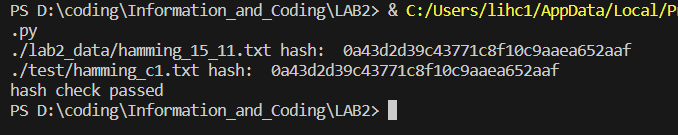
\includegraphics[width=12cm]{./pic/1-1.png}		
        \caption{c1:编码后文件哈希比较}
    \end{figure}

    验证每个编码结果在使用我的程序解码后与原始数据相同,结果如图:
    \begin{figure}[H]
        \centering
        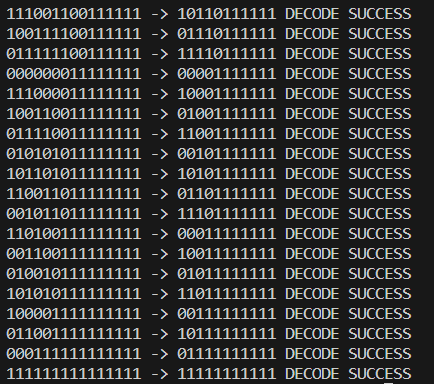
\includegraphics[width=8cm]{./pic/1-2.png}		
        \caption{c1:解码后与原始数据相同}
    \end{figure}

    验证随机修改每个编码结果中的一位,并使用程序解码,解码后的结果与原始数据相同。结果如图:
    \begin{figure}[H]
        \centering
        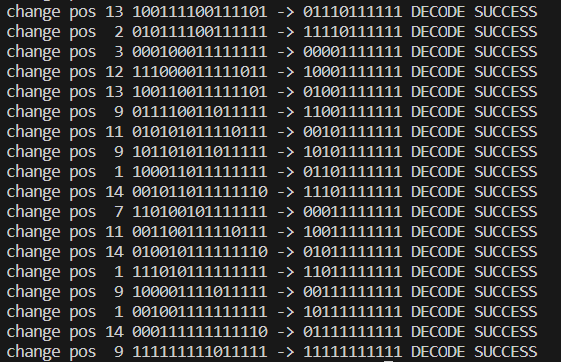
\includegraphics[width=8cm]{./pic/1-3.png}		
        \caption{c1:引入一位错误后正确解码}
    \end{figure}
    
    
\section*{C2:在一台资源紧张的嵌入式设备实现[255,247]汉明码,使用矩阵乘法,会出什么问题?}

\subsection*{1.时间复杂度}

矩阵乘法的时间复杂度较高,通常为 $O(n^3)$,其中 $n$ 是矩阵的维度。对于较大的汉明码,例如[255, 247],计算生成矩阵与消息向量的乘积将需要较长的时间。在资源受限的嵌入式设备上,这可能会导致处理时间过长,不符合实时性要求。

\subsection*{2.空间复杂度}

使用矩阵乘法需要存储生成矩阵的完整形式,这将占用大量的存储空间。对于[255, 247]汉明码,生成矩阵的维度为 247 × 255,需要存储大量的矩阵元素。在资源受限的嵌入式设备上,存储空间通常是有限的,因此这种方法可能无法满足存储空间的要求。

\section*{OP1:对[7,4]汉明码,证明上述编码构造方法等价。}

对消息$\bm{d} = d_0d_1d_2d_3$进行编码得到$p_0p_1d_0p_2d_1d_2d_3$,使用奇偶检验方法实现汉明码部分可知:
    
    $$
    \begin{aligned}
    p_0 &= d_0 \oplus d_1 \oplus d_3\\
    p_1 &= d_0 \oplus d_2 \oplus d_3\\
    p_2 &= d_1 \oplus d_2 \oplus d_3
    \end{aligned}
    $$
    
    在[7,4]汉明码中,生成矩阵G可以计算得到为:
    $$
    G =
    \begin{pmatrix}
    1 & 1 & 1 & 0 & 0 & 0 & 0 \\
    1 & 0 & 0 & 1 & 1 & 0 & 0 \\
    0 & 1 & 0 & 1 & 0 & 1 & 0 \\
    1 & 1 & 0 & 1 & 0 & 0 & 1 
    \end{pmatrix}
    $$

    则可以计算:
    $$
    \begin{aligned}
    \bm{r} &= \bm{d} \times G \\
           &= (d_0 + d_1 + d_3, d_0 + d_2 + d_3, d_0, d_1 + d_2 + d_3, d_1, d_2, d_3)
    \end{aligned}
    $$

    因此两种构造方法等价。


\section*{OP2:证明:这种构造方式与优化前的构造方式等价。}
    
    在[7,4]汉明码中,数据位分别为第$3,5,6,7$位,使用二进制表达分别为第$011, 101, 110, 111$位。因此使用第二种编码方式时,计算得到的校验位$b_0b_1b_2$时,取出二进制表达的低0、1、2位,则表达式分别为:

    $$
    \begin{aligned}
    b_0 &= d_0 \& 1 \oplus d_1 \& 1 \oplus d_2 \& 0 \oplus d_3 \& 1 = p_0\\
    b_1 &= d_0 \& 1 \oplus d_1 \& 0 \oplus d_2 \& 1 \oplus d_3 \& 1 = p_1\\
    b_2 &= d_0 \& 0 \oplus d_1 \& 1 \oplus d_2 \& 1 \oplus d_3 \& 1 = p_2
    \end{aligned}
    $$

    因此两种构造方式等价。

\section*{C3:使用奇偶校验方法实现[15,11]汉明码}
    \subsection*{1.算法过程}
    使用简单的奇偶校验位进行Hamming码的编码和解码,相比于上一部分,这个方法不使用矩阵,而是直接在编码和解码过程中操作位。

    编码过程为:首先检查原始数据长度是否正确,然后生成校验位的索引,将每个校验位对应的信息位的索引存储在index列表中。接下来,将信息位放入结果列表中对应的位置,然后计算校验位并将其放入结果列表中。最后,将结果列表转换为字符串并返回。

    解码过程为:首先检查编码数据长度是否正确,然后将编码数据转换为整数列表,并记录所有为1的位的索引。通过将所有为1的位的索引进行异或操作,得到错误位的索引。如果存在错误位,则将错误位的值进行翻转。从纠正后的数据中提取出原始数据,将原始数据转换为字符串并返回。

    \subsection*{2.编程实现}
    "HammingCheck.py"文件中的hamming\_check类实现了编码和解码的功能。

    验证过程可以运行"c3\_check.py"文件。首先验证码表中的每个原始数据在使用我的程序编码后与编码结果相同,采用哈希函数验证的方法,结果如图,验证成功:
    \begin{figure}[H]
        \centering
        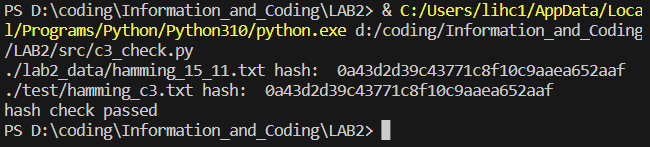
\includegraphics[width=12cm]{./pic/2-1.png}		
        \caption{c3:编码后文件哈希比较}
    \end{figure}

    验证每个编码结果在使用我的程序解码后与原始数据相同,结果如图:
    \begin{figure}[H]
        \centering
        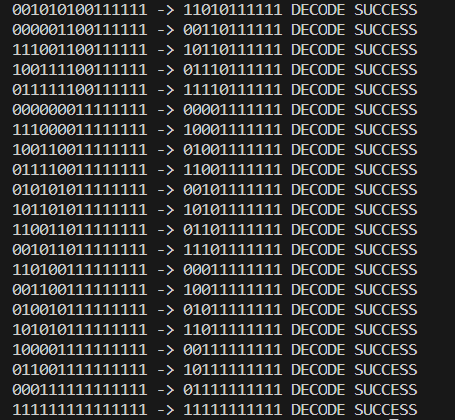
\includegraphics[width=8cm]{./pic/2-2.png}		
        \caption{c3:解码后与原始数据相同}
    \end{figure}

    验证随机修改每个编码结果中的一位,并使用程序解码,解码后的结果与原始数据相同。结果如图:
    \begin{figure}[H]
        \centering
        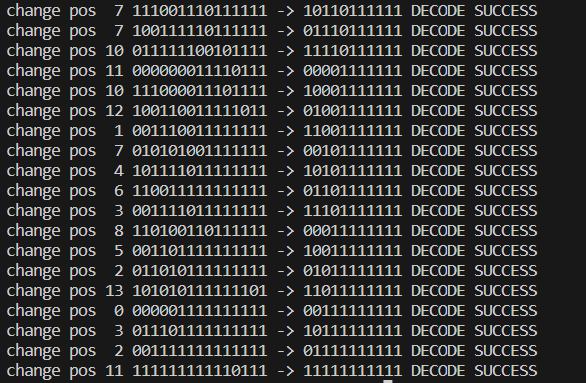
\includegraphics[width=8cm]{./pic/2-3.png}		
        \caption{c3:引入一位错误后正确解码}
    \end{figure}


\section*{C4:在一台资源非常紧张的嵌入式设备实现(255,247)汉明码,使用上述的奇偶校验观点会有什么优势?}

\subsection*{1.时间复杂度}

奇偶校验方法的计算复杂度较低。在构造汉明码时,只需遍历消息比特并计算校验比特的值,这个过程的时间复杂度为 $O(k)$,其中 $k$ 是消息比特的数量(247)。相比之下,矩阵方法的时间复杂度为 $O(n^3)$,其中 $n$ 是码字长度(255),因此奇偶校验方法更快。

\subsection*{2.空间复杂度}

奇偶校验方法只需要额外存储一个校验比特,相对于矩阵方法而言,所需的存储空间更少。在(255, 247)汉明码中,只需存储一个校验比特的值,而不需要存储整个生成矩阵。这对于资源受限的嵌入式设备来说是一个重要的优势。


\section*{C5:程序测试}
    \subsection*{C5.1: 1 比特错误}
    
    用于c5测试的代码文件分别为"c5\_encode.py"和"c5\_decode.py",分别实现编码和解码操作。
    
    C5.1 的测试结果为:
    \begin{figure}[H]
        \centering
        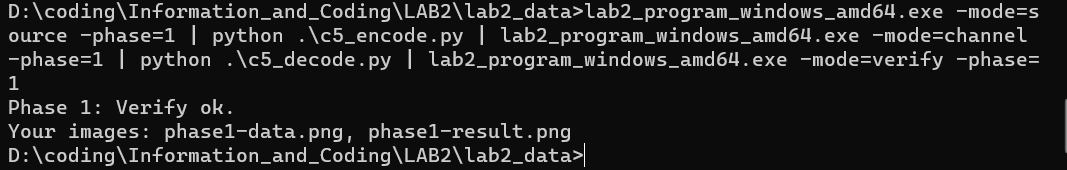
\includegraphics[width=12cm]{./pic/3-1.png}		
        \caption{c5.1 运行结果}
    \end{figure}

    生成的图片为:
    \begin{figure}[H]
    \centering
    \begin{minipage}[t]{0.45\textwidth}
    \centering
    
\includegraphics[width=5cm]{./pic/phase1-data.png}
    \caption{phase1-data图片}
    \end{minipage}
    \hfill
    \begin{minipage}[t]{0.45\textwidth}
    \centering
    
\includegraphics[width=5cm]{./pic/phase1-result.png}
    \caption{phase1-result图片}
    \end{minipage}
    \end{figure}

    信源数据和解码后的图片相同,是因为虽然每 15 个比特都会有 1 个比特出错,但是[15,11]汉明码可以纠正1比特的错误,因此数据不变。


    \subsection*{C5.2: 2 比特错误}
    C5.2 的测试结果为:
    \begin{figure}[H]
        \centering
        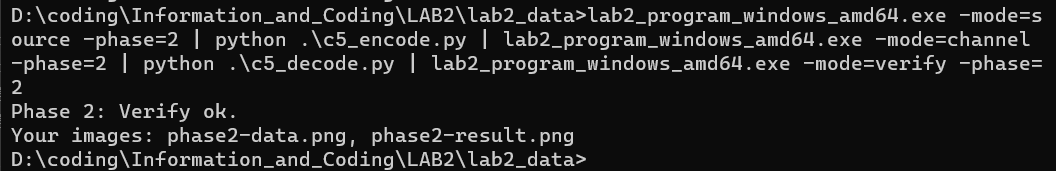
\includegraphics[width=12cm]{./pic/3-2.png}		
        \caption{c5.2 运行结果}
    \end{figure}

    生成的图片为:
    \begin{figure}[H]
    \centering
    \begin{minipage}[t]{0.45\textwidth}
    \centering
    
\includegraphics[width=5cm]{./pic/phase2-data.png}
    \caption{phase2-data图片}
    \end{minipage}
    \hfill
    \begin{minipage}[t]{0.45\textwidth}
    \centering
    
\includegraphics[width=5cm]{./pic/phase2-result.png}
    \caption{phase2-result图片}
    \end{minipage}
    \end{figure}

    信源数据和解码后的图片有差异,因为[15,11]汉明码只可以纠正1比特的错误而不能纠正2比特。图中有些分组仍然被正确编码译码了,例如第一组。

    \subsection*{C5.3: 突发错误}
    C5.3 的测试结果为:
    \begin{figure}[H]
        \centering
        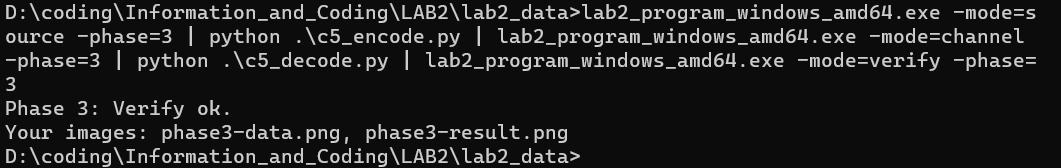
\includegraphics[width=12cm]{./pic/3-3.png}		
        \caption{c5.3 运行结果}
    \end{figure}

    生成的图片为:
    \begin{figure}[H]
    \centering
    \begin{minipage}[t]{0.45\textwidth}
    \centering
    
\includegraphics[width=5cm]{./pic/phase3-data.png}
    \caption{phase3-data图片}
    \end{minipage}
    \hfill
    \begin{minipage}[t]{0.45\textwidth}
    \centering
    
\includegraphics[width=5cm]{./pic/phase3-result.png}
    \caption{phase3-result图片}
    \end{minipage}
    \end{figure}

    信源数据和解码后的图片有差异,因为[15,11]汉明码只可以纠正1比特的错误而不能纠正更多。在出现多个错误位时将不能正确译码。

\section*{OP4: 2 比特错误检测}

\subsection*{OP4.1: 证明上述的算法能正确纠正一个错误,检出两个错误}

    对消息$\bm{d} = d_0d_1d_2d_3$进行编码得到$\bm{m} = p_0p_1d_0p_2d_1d_2d_3$,由上述使用奇偶检验方法实现汉明码部分可知:
    
    $$
    \begin{aligned}
    p_0 &= d_0 \oplus d_1 \oplus d_3\\
    p_1 &= d_0 \oplus d_2 \oplus d_3\\
    p_2 &= d_1 \oplus d_2 \oplus d_3
    \end{aligned}
    $$

    在最后加一位奇偶校验位$G$,计算方法为$\bm{m}$中1的个数,即将$\bm{m}$中数字诸位异或得到额外的奇偶校验位放在最后。
 
    发生2比特错误时,由于每个校验位只负责监测与其相关的信息位的奇偶性,如果发生两个错误,则会导致多个校验位的奇偶性不匹配。通过检查多个校验位的奇偶性,我们可以确定出现了两个错误的事实,但是无法准确确定是哪两个比特位发生了错误。因此,算法能够检测到两个错误的存在。

\subsection*{OP4.2: 编程实现[16,11]扩展汉明码}

    编程实现过程中使用了C3部分的汉明码实现代码,在此基础上进行扩展,程序文件为"HammingCheckEnhance.py"。

    encode方法用于对给定的消息进行编码,首先调用hamming\_check对象的encode方法对消息进行编码,然后计算校验位,将校验位拼接到编码后的结果中,并返回最终的编码结果。

    decode方法用于对给定的编码消息进行解码,首先检查消息长度是否正确,然后计算校验位,调用hamming\_check对象的decode方法对消息进行解码,得到解码结果和错误位数。根据错误位数和校验位的值,判断出现的错误类型,并返回相应的结果。

    如果检测发现产生1比特错误或者没有产生错误,则返回正确的解码结果;如果检测到2比特的编码错误,则返回提示,并无法正确解码。

    测试过程中随机引入5组1比特错误和5组2比特错误,测试结果均正确,测试结果如图:
    \begin{figure}[H]
        \centering
        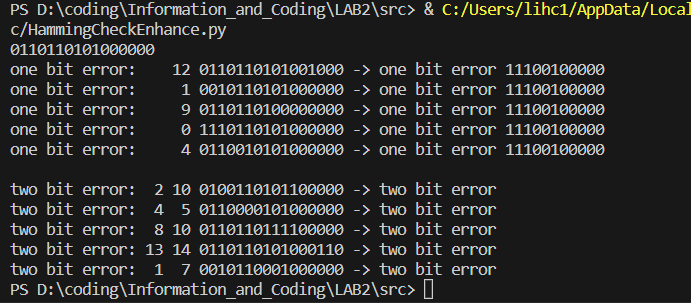
\includegraphics[width=12cm]{./pic/4-1.png}		
        \caption{OP4.2 运行结果}
    \end{figure}


\end{document}